\documentclass{article}
\usepackage[utf8]{inputenc}
\usepackage{amsmath}
\usepackage{amssymb}
\usepackage{tikz}

\begin{document}
\subsection*{Daniel Bustos, BFS raiz v es v-Geodesico}
Un árbol generador $T$ de un grafo $G$ es $v$-geodésico si la distancia entre $v$ y $w$ en $T$ es igual a la distancia entre $v$ y $w$ en $G$ para todo $w \in V(G)$. Demostrar que todo árbol BFS de $G$ enraizado en $v$ es $v$-geodésico.

Probémoslo: Si $T$ es un árbol BFS de $G$ enraizado en $v\implies T$ es $v$-geodésico.

Hagamos inducción en las distancias a la raíz $r$. Vamos a usar (pero no demostrar) el siguiente lema:

\textbf{Lema:} Sea $T$ un árbol BFS desde raíz de un (di)grafo $G$. Si el nivel de $v$ es menor al nivel de $w$ en $T$, entonces $v$ se procesó antes que $w$ por BFS.

Ahora si empecemos la inducción:

$P(n)$ := Para todo nodo a distancia $n$ de la raíz $r$ en $T$, su distancia en $G$ es igual a su distancia en $T$: $d_T(r,v') = n \leftrightarrow d_G(r,v') = n$.

\textbf{Caso base:} $P(0)$, vale trivialmente, ya que la distancia en BFS a la raíz es $0$, ya que es el primer nodo en ser procesado.\\

\textbf{Paso Inductivo:}
\textbf{H.I.} : $\exists l_0 \in \mathbb{N}$ tal que $\forall l' \leq l_0$ vale $P(l')$.\\

\textbf{Q.V.Q.} $P(l_0) \rightarrow P(l_0 + 1)$.
\begin{itemize}
    
\item Consideremos el camino minimo $P = r,v_1,v_2,\ldots,v_{l+1}$ en G. Sabemos que $d_G(r,v_{l+1}) = n + 1$ y  por H.I. que el nodo $v_l$ está en el nivel $l$ del árbol BFS.\\

\item Cuando BFS mira este vértice, toma a todos sus vecinos, dentro de los cuales debe estar $v_{l+1}$, si no fue marcado por BFS, este lo toma y vale $P(l_0 + 1)$. 
\item Caso contrario quiere decir que el nodo ya fue marcado por BFS , lo que quiere decir que $\exists$ un vertice w con altura $< l_0$ tal que $v_{l_0+1} \in N(w)$. Como w cumple la H.I, quiere decir que $d_T(r,w) = d_G(r,w)$. Luego tenemos ya que $d_G(r,w) < l $ vale lo siguiente :

\[d_G(r,w) + 1 = d_T(r,w) + 1 (*) \leq l_0 + 1 = d_G(r,v_{l_{0 + 1}} )\]
Con la distancia $(*)$ representando $d_T(r,v_{l_0 + 1})$ cuando pasa por $w$.
Ademas siempre vale que la distancia en el arbol T debe ser mayor o igual a la distancia en G, por el funcionamiento de BFS. 
Entonces se puede deducir lo siguiente: 
    \[d_T(r,v_{l_0 + 1}) \leq v_{l_{0 + 1 }} \land  \ d_T(r,v_{l_0 + 1}) \geq v_{l_{0 + 1 }}    \]
    \[ \implies d_T(r,v_{l_0 + 1}) = l_{0 + 1 }\]
Que es lo que queriamos ver $\square$


\end{itemize}

Veamos la falsedad de: Si \( T \) es \( v' \)-geodésico \(\implies\) \( T \) es un árbol BFS de \( G \) enraizado en \( v' \). Para el contraejemplo, tomemos el siguiente grafo: \( (v,w)(w,z) \). Claramente, si construimos el árbol BFS desde cualquiera de los tres, siempre será \( w/z/v \)-geodésico, sin necesariamente ser la raíz. Esto demuestra que no vale la vuelta de la propiedad.

\begin{figure}
    \centering
    \begin{minipage}{0.45\textwidth}
        \centering
        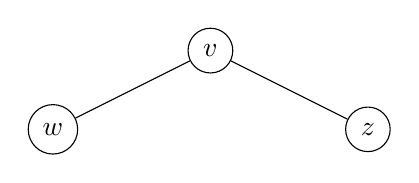
\begin{tikzpicture}
            \node[circle,draw] (v1) at (0,1) {$v$};
            \node[circle,draw] (w1) at (-2,0) {$w$};
            \node[circle,draw] (z1) at (2,0) {$z$};
            
            \draw (v1) -- (w1);
            \draw (v1) -- (z1);
        \end{tikzpicture}
       
    \end{minipage}
    \hfill
    \begin{minipage}{0.45\textwidth}
        \centering
        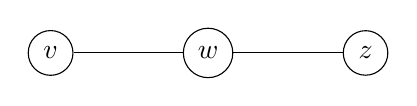
\begin{tikzpicture}
            \node[circle,draw] (v2) at (0,0) {$v$};
            \node[circle,draw] (w2) at (2,0) {$w$};
            \node[circle,draw] (z2) at (4,0) {$z$};
            
            \draw (v2) -- (w2);
            \draw (w2) -- (z2);
        \end{tikzpicture}
       
    \end{minipage}
     \caption{La distancia no cambia en ninguno de los nodos, sin necesariamente ser la raíz del árbol.}
\end{figure}


\end{document}
